\chapter[Dise\~no]{
  \label{chp:diseno}
  DISE\~NO
}
\thispagestyle{numberingStyle}
\pagestyle{numberingStyle}


\section{Arquitectura del sistema}
La arquitectura empleada en el sistema será una arquitectura en capas, una de las técnicas de diseño más usadas en las ciencias de la computación. La arquitectura basada en capas es una especialización de la arquitectura cliente-servidor donde la carga de trabajo se divide en diferentes capas con un reparto claro de las funciones.

En esta arquitectura, una capa inferior proporciona un servicio a otra copa superior. El servicio ofrecido se define mediante un contrato de servicio. De esta forma, se consigue independizar el software de ambas capas y los cambios de implementación en una de ellas no tienen repercusión sobre las demás.

Partiendo que la aplicación será accesible desde dispositivo móvil y navegador web, se presentará una solución al diseño basada en dos alternativas de la arquitectura basada en capas: la arquitectura en 3 capas y la arquitectura en 4 capas.


\subsection{Arquitectura en 3 capas físicas}
En este sistema de arquitectura, se diferencian tres capas físicas que cumplen funciones diferentes.

\begin{figure}[H]

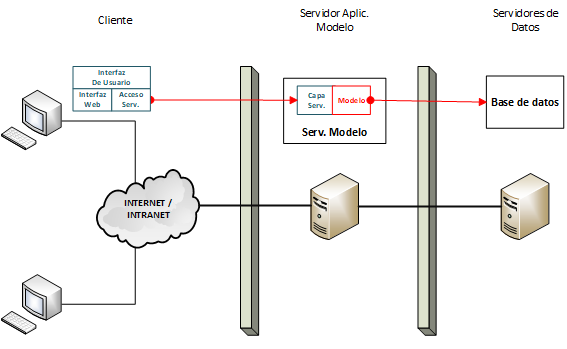
\includegraphics[
   keepaspectratio=true
]{./05_Diseno/arq3capas.png}
\caption{Diagrama arquitectura en tres capas}
\end{figure}

\begin{itemize}
	\item \textbf{Capa Física - Servidor de Datos: } Es la capa encargada de gestionar el almacenamiento de los datos.
	\item \textbf{Capa Física - Servidor Aplicación Modelo:} Formada por las siguientes capas lógicas.
	\begin{itemize}
		\item \textbf{Capa Modelo:} Es la encargada implementar las funcionalidades de la aplicación y mantener la comunicación con el servidor de datos realizando las acciones relacionadas con el acceso a los datos. Comúnmente, se subdivide en dos, la capa de acceso a datos, para la conexión con el servidor de datos, y la capa lógica de negocio, para la implementación de los casos de uso.
		\item \textbf{Capa Servicios: } Sirve de enlace entre la interfaz de usuario y la capa modelo. 
	\end{itemize}		
	\item \textbf{Capa Física - Cliente: } Dividida en las siguientes capas lógicas.
	\begin{itemize}
		\item \textbf{Capa de Acceso al Servicio: } Capa encargada de acceder e invocar a los métodos de la capa de servicios del modelo.
		\item \textbf{Capa Interfaz de Usuario: } Interfaz gráfica final que se instala en las máquinas cliente y dispositivos finales.
	\end{itemize}
\end{itemize}



\subsection{Arquitectura en 4 capas físicas}
En esta alternativa, se añade una capa intermedia entre el cliente y el modelo que actúa de servidor de aplicaciones y que proporciona la interfaz web para clientes que accedan desde navegador web.

\begin{figure}[!h]

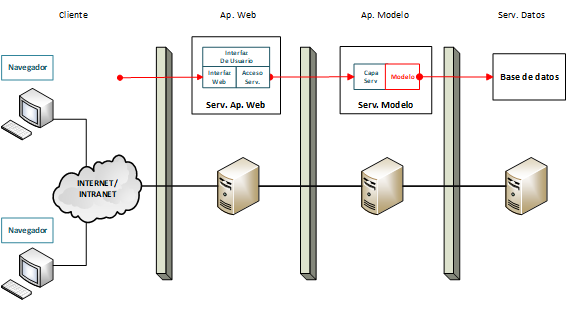
\includegraphics[
   keepaspectratio=true
]{./05_Diseno/arq4capas.png}
\caption{Diagrama arquitectura en cuatro capas}
\end{figure}

Un navegador, para acceder a la aplicación, necesitará de un servidor de aplicaciones que le proporcione la interfaz web. Incorporar esta interfaz dentro del servidor de aplicaciones visto en la arquitectura anterior haría que este y el modelo estén fuertemente acoplados, impidiendo que puedan ser construidos con tecnologías diferentes.

Por ello, con esta arquitectura se pretende hacer ese desacople consiguiendo que múltiples aplicaciones puedan invocar al modelo, independientemente de que sean con interfaz gráfica o mediante navegador, sin necesidad de replicar el código del modelo en cada aplicación.

En consecuencia, analizados los requisitos del sistema y conociendo las necesidades del mismo, se diseñará un sistema basado en una arquitectura de cuatro capas desde el punto de vista de un cliente web, y de tres capas, desde el punto del cliente móvil.


\subsection{Arquitectura completa del sistema}

\begin{figure}[!h]

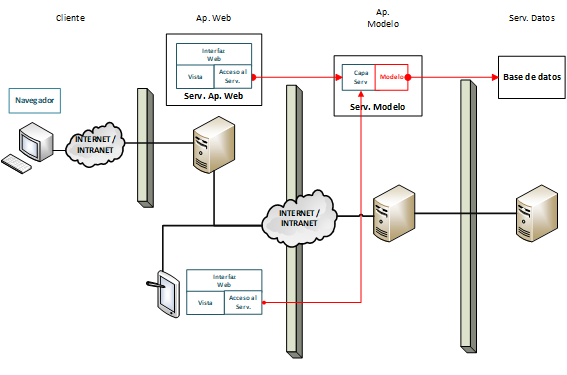
\includegraphics[
   keepaspectratio=true
]{./05_Diseno/arqsistema.png}
\caption{Diagrama arquitectura completa del sistema}
\end{figure}

Como se puede observar en el diagrama, el sistema sigue una arquitectura global en cuatro capas.

Al tener la aplicación modelo desacoplada de la aplicación web, la capa de servicios debe servir de enlace entre la capa modelo y la interfaz de usuario. Ese enlace lo ofrece mediante unos servicios web, que exponen a la capa superior, las funcionalidades implementadas en la capa modelo.

La capa modelo accederá a diferentes servicios de datos. La base de datos permitirá almacenar la información relevante de la aplicación mientras que las fuentes de datos externas, Foursquare y Google, servirán para consultas de lugares y cálculos de distancias, respectivamente. A mayores, la aplicación web y la aplicación cliente móvil, harán uso directo del servicio de datos de Google para la visualización de mapas (Línea azul en la figura).

Por su parte, en las aplicaciones cliente, la interfaz web del servidor de aplicaciones y la interfaz del cliente móvil, siguen el patrón de arquitectura Modelo-Vista-Controlador (MVC) y Modelo-Vista-VistaModelo (MVVM), respectivamente. En ellas, el modelo no se encuentra implementado en la propia aplicación, sino que es accedido a través de la capa de acceso a los servicios. De esta forma, ambas aplicaciones finales, invocan al modelo sin necesidad de tenerlo replicado.



\section{Diseño físico de los datos}
\subsection{Modelo Entidad-Relación}
\begin{figure}[H]
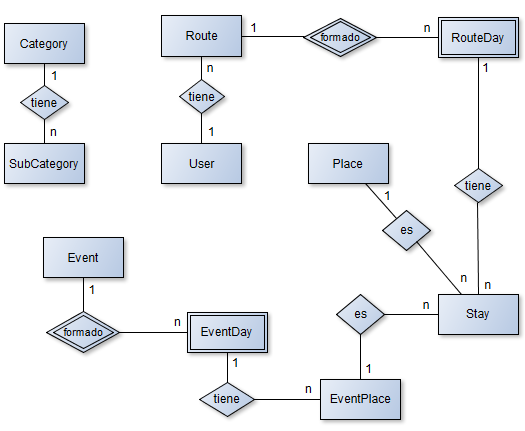
\includegraphics[
   keepaspectratio=true
]{./05_Diseno/ER.png}
\caption{Diagrama Entidad-Relación}
\end{figure}

En el apéndice se incluye un diagrama Entidad-Relación completo, incluyendo entidades y atributos.


\section{Capa Modelo}
Esta capa es la encargada de implementar la lógica de negocio de la aplicación, lo que implica el manejo de las entidades persistentes y el acceso a los datos. Como podemos observar en la Figura 7.5, y debido a la arquitectura establecida, el modelo estará compuesto por la capa de acceso a datos y la capa de lógica de negocio.

\begin{figure}[H]
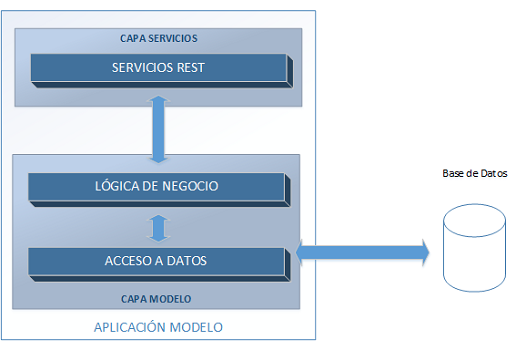
\includegraphics[
   keepaspectratio=true
]{./05_Diseno/disenomodelo.png}
\caption{Diagrama diseño modelo}
\end{figure}


\subsection{Diseño módulo acceso a datos}
En la capa de acceso a datos se definirán el conjunto de entidades persistentes que manejará la aplicación y se empleará el patrón de diseño Data-Access-Object (DAO) para abstraer la persistencia de las entidades, así como la fuente de datos empleada.

Por cada entidad persistente existirá un DAO encargado de gestionar la comunicación con la fuente de datos empleada.

\subsubsection*{Diagrama clases persistentes}
\begin{figure}[H]
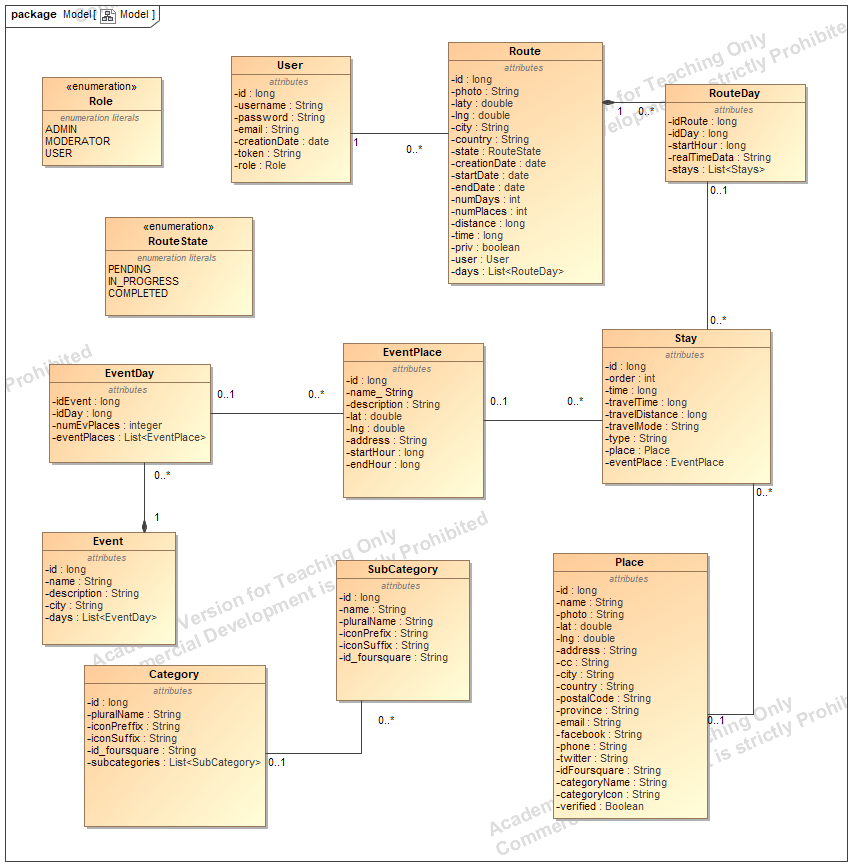
\includegraphics[
   keepaspectratio=true
]{./05_Diseno/disenoclases.png}
\caption{Diagrama clases persistentes}
\end{figure}

En el diagrama se muestran las clases persistentes que manejará la aplicación. A continuación, se detallará brevemente, el significado y funcionalidad de cada una:

\begin{itemize}
	\item \textbf{User: }Es la clase encargada de representar la información de los usuarios registrados en la aplicación.
	\item \textbf{Role: } Enumerado con los roles disponibles para un usuario: \textit{ADMIN, MODERATOR y USER}.
	\item \textbf{Route: }Clase encargada de guardar la información sobre las rutas creadas por los usuarios. Las rutas están compuestas por \textit{RouteDays}.
	\item \textbf{RouteDay: }Clase con una relación fuerte de composición con la clase \textit{Route}. Su tiempo de vida está condicionada por la vida de la clase que la incluye. Mantiene la información para cada uno de los días que componen la duración de una ruta.
	\item \textbf{RouteState: }Enumerado con los diferentes estados por los que pasa una ruta en el tiempo: \textit{PENDING, IN\_PROGRESS y COMPLETED}.
	\item \textbf{Stay: }Entidad con la funcionalidad de almacenar las visitas que decida hacer un usuario en un día de una ruta determinada. La visita, puede ser a lugares obtenidos de la fuente externa (Foursquare) o a eventos gestionados por la propia aplicación.
	\item \textbf{Place: }Entidad que registra y almacena los detalles sobre los lugares extraídos de la fuente externa.
	\item \textbf{Event: }Es la clase encargada de representar los eventos dados de alta en el sistema. Los eventos están compuestos por \textit{EventDays}.
	\item \textbf{EventDay: }Clase con una relación fuerte de composición con la clase \textit{Event}. Su tiempo de vida está condicionada por la vida de la clase que la incluye. Mantiene la información para cada uno de los días que componen al evento.
	\item \textbf{EventPlace: }Es la clase donde se maneja toda la información sobre las distintas ubicaciones y actividades que incluye un día determinado del evento.
	\item \textbf{Category: }Clase que almacena la información relevante a las categorías sobre las que se filtran los lugares obtenidos de Foursquare.
	\item \textbf{SubCategory: }Establece una jerarquía con la clase anterior. Almacena las categorías que son un subtipo de una categoría determinada.
\end{itemize}


\subsubsection*{Patrón de diseño DAO}
Este patrón de diseño intenta desacoplar el acceso a los datos de su almacenamiento subyacente. Los datos persistentes, actualmente, dependen en gran medida del tipo de base de datos utilizada: base de datos relacional, base de datos orientada a objetos, archivos planos... siendo las bases de datos relacionales las más utilizadas. 

Partiendo de que los accesos a diferentes tipos de bases de datos se realizan de manera muy diferente, utilizar este patrón en lugar de acceder directamente a la fuente de datos, nos permite pasar de un tipo de fuente de datos a otro diferente sin tener que realizar modificaciones en la lógica de negocio.


\begin{figure}[H]
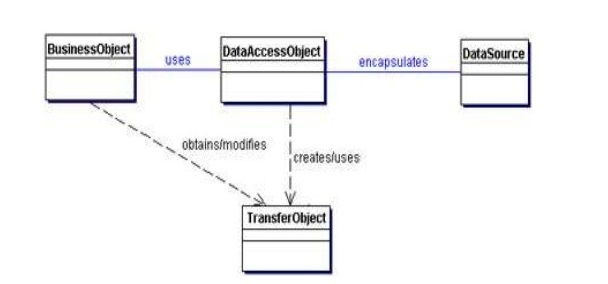
\includegraphics[
   keepaspectratio=true
]{./05_Diseno/patrondao.jpg}
\caption{Diagrama patrón de diseño DAO}
\end{figure}

En la Figura 7.7 se muestra un pequeño diagrama con los elementos participantes en este patrón de diseño.

\begin{itemize}
	\item \textbf{Business Object: }Representa la clase con la lógica de negocio. Es la responsable de saber qué y cómo modificar el contenido de los datos pero no cómo almacenarlo.
	\item \textbf{Data Access Object: }Se encarga de ocultar la fuente de datos real de manera que el objeto con la lógica de negocio (Business Object) se comunica con este en vez de hacerlo directamente con el objeto de acceso a los datos.
	\item \textbf{DataSource: }Es la clase encargada de obtener las conexiones a la base de datos.
	\item \textbf{Transfer Object: }Es el objeto que se utiliza para transferir el contenido de los datos reales, del \textit{Data Access Object} al objeto de negocio \textit{Business Object}. Representa los datos almacenados en la base de datos.
\end{itemize}


\subsubsection*{Diseño de los DAOs}
\begin{figure}[H]
\centering
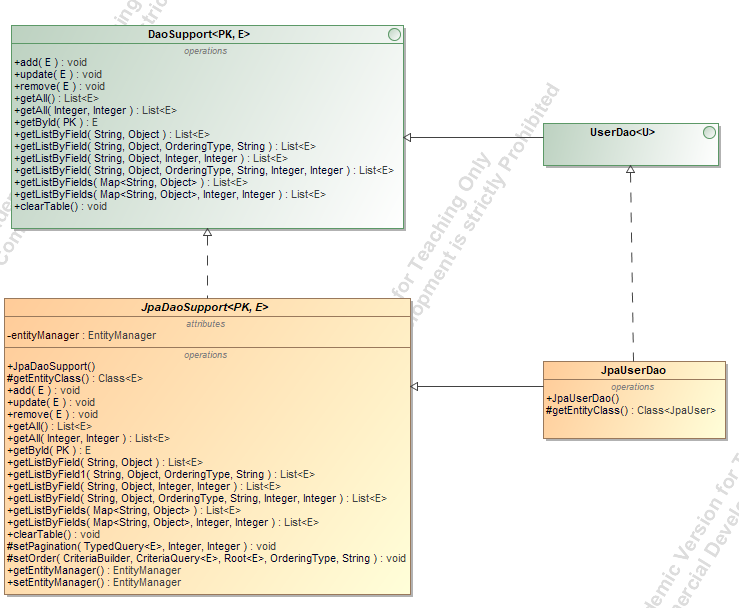
\includegraphics[
   keepaspectratio=true
]{./05_Diseno/userdao.png}
\caption{Ejemplo UserDao}
\end{figure}

En la figura 7.8 se muestra un esquema en el que se define e implementa un DAO genérico que proporciona las principales operaciones de acceso a datos, permitiendo que las definiciones de DAOs, que extiendan a este DAO genérico, tengan las operaciones básicas sin necesidad de redefinirlas ni implementarlas. Del mismo modo, en los DAOs que extiendan el DAO genérico, también se podrán definir e implementar funcionalidades específicas para cada uno de ellos. Este ejemplo, del DAO de la entidad \textit{User}, se compone de:

\begin{itemize}
	\item \textbf{DaoSupport: } Interfaz que define una serie de métodos y operaciones sobre los datos.
	\item \textbf{JpaDaoSupport: } Clase genérica que implementa las funciones de la interfaz anterior.
	\item \textbf{UserDao: } Definición del DAO específico para la entidad \textit{User}. Extiende las funcionalidades de la interfaz \textit{DaoSupport} y en este caso, no incluye ningún más.
	\item \textbf{JpaUserDao: } Implementación de \textit{UserDao} que extiende la implementación de las funciones de la clase genérica. 
\end{itemize}

Este esquema se repite con todas las entidades, exceptuando aquellas que necesitan de una relación con otra entidad para existir. Por ejemplo, la entidad \textit{RouteDay} necesita de \textit{Route} para existir, por lo que su identificador es dependiente de la otra entidad. Para este tipo de entidades, que no pueden seguir las definiciones del DAO genérico explicado anteriormente por estar diseñado únicamente para entidades formadas por identificadores de un único atributo, se presenta una solución particular para cada entidad, donde cada DAO define e implementa sus funcionalidades necesarias. 

El diseño de los diferentes DAOs definidos en la aplicación pueden consultarse en el apéndice.


\newpage
\subsection{Diseño módulo lógica de negocio}
En este módulo o subcapa es donde se implementan y desarrollan los casos de uso previamente especificados.

En el diseño de los servicios ofrecidos se utilizará el patrón de diseño Fachada. Con este patrón, se crearán una serie de servicios que agruparán y gestionarán un conjunto determinado de entidades y componentes ofrecidos por la capa de acceso a datos. Estos servicios ofrecerán una serie de funcionalidades abstrayendo la complejidad de implementación y de dependencia con demás componentes.

\subsubsection*{Patrón Fachada}
El propósito del patrón de diseño Fachada es proporcionar una interfaz unificada para un conjunto de interfaces en un subsistema. Se define una interfaz de nivel superior lo que permite hacer el subsistema más fácil de utilizar.

\begin{figure}[H]
\centering
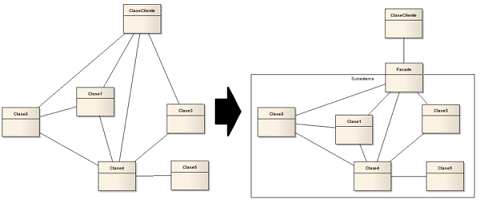
\includegraphics[
   keepaspectratio=true
]{./05_Diseno/patronfacade.png}
\caption{Diagrama patrón de diseño Fachada}
\end{figure}

Estructurar un sistema en subsistemas ayuda a reducir la complejidad. Uno de los objetivos más comunes de diseño es minimizar la comunicación y las dependencias entre los subsistemas. Esto se puede lograr haciendo uso de este patrón.

Como podemos observar en la Figura 7.9, utilizando el patrón fachada se proporciona una interfaz única de acceso que se encargar de gestionar las comunicaciones y dependencias necesarias con otros módulos o subsistemas para realizar sus funcionalidades. Permite abstraer al cliente de cómo se gestionan las comunicaciones con los diferentes módulos.


\subsubsection*{Diseño de los servicios}
\begin{figure}[H]
\centering
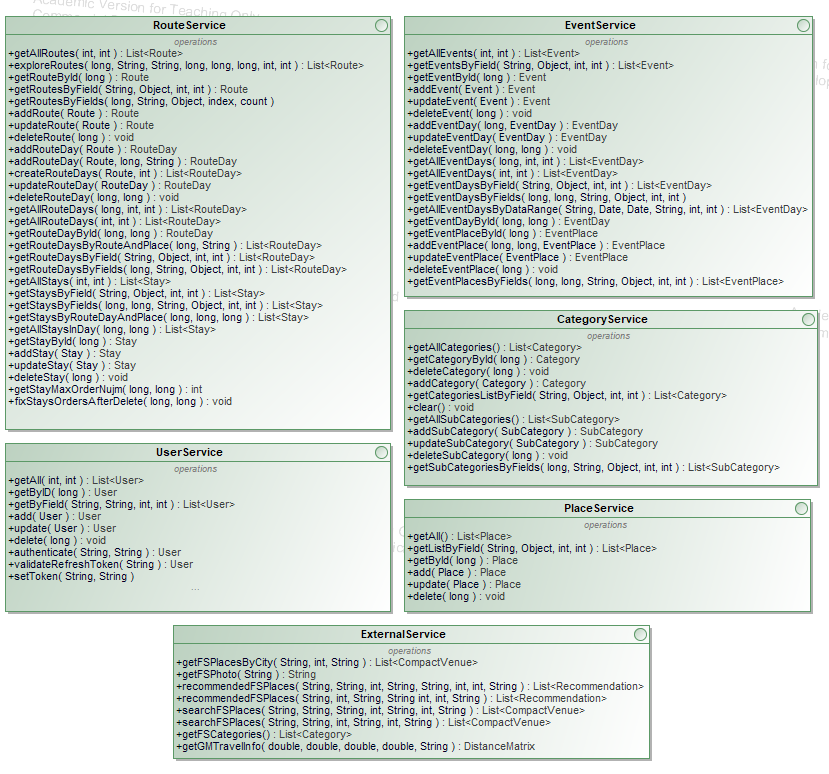
\includegraphics[
   keepaspectratio=true
]{./05_Diseno/disenoservicios.png}
\caption{Diagrama diseño servicios}
\end{figure}

En la Figura 7.10 podemos ver el diseño de los servicios que implementarán las funcionalidades de la aplicación. Se detallan brevemente a continuación:

\begin{itemize}
	\item \textbf{RouteService: }Servicio encargado de implementar los casos de uso o funcionalidades referentes a las rutas. Gestionan tanto las propias rutas como su composición por días y las visitas incluidas en cada día.
	\item \textbf{EventService: }Este servicio es el encargado de la gestión de los eventos en la aplicación. Al igual que con el anterior servicio, este incluye las funcionalidades para gestionar la composición por días y los lugares o ubicaciones específicas que existan dentro de un mismo evento.
	\item \textbf{UserService: }Ofrece los casos de uso referente a la entidad usuarios. Incluye desde el manejo de los datos sobre los usuarios hasta las funcionalidades de autenticación.
	\item \textbf{CategoryService: } Es el servicio encargado de administrar las categorías.
	\item \textbf{PlaceService: }Presenta las funcionalidades necesarias para gestionar los lugares que se registran en la aplicación.
	\item \textbf{ExternalService: }Es el servicio encargado de ofrecer las funciones que requieren de una comunicación con fuentes de datos externos. En este caso, se proporcionará una implementación que hará uso de las APIs de Foursquare y de Google Maps.
\end{itemize}

\subsubsection*{Diagrama ejemplo patrón fachada}
\begin{figure}[H]
\centering
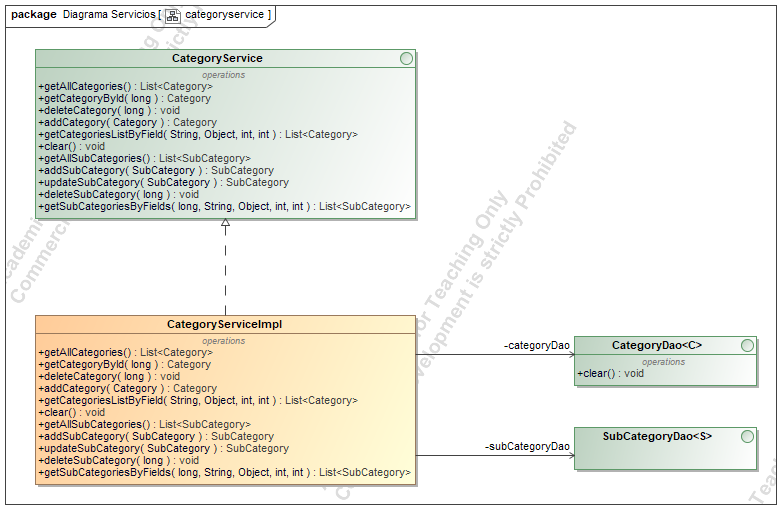
\includegraphics[
   keepaspectratio=true
]{./05_Diseno/categoryservice.png}
\caption{Ejemplo \textit{CategoryService}}
\end{figure}

En la figura 7.11, podemos ver el ejemplo de un servicio concreto, en este caso \textit{CategoryService}. En este ejemplo, podemos observar la definición del servicio a través de la interfaz \textit{CategoryService} y donde su implementación es la encargada de gestionar las comunicaciones con los diferentes módulo y subsistemas, en este caso, con los DAOs de las entidades \textit{Category} y \textit{SubCategory}.



\section{Capa servicios}
La capa de servicios ofrecerá las funcionalidades de la capa modelo a través de recursos accesibles por la red, mediante peticiones HTTP. Se proporcionará una implementación de la capa de servicios siguiendo el  estilo arquitectónico Representational State Transfer (REST) mediante el uso del API de programación JAX-RS.

Se utilizará el patrón de diseño Data Transfer Object (DTO).

\subsubsection*{Patrón de diseño DTO}
Es un patrón de diseño que se utiliza para transferir varios atributos entre un cliente y un servidor, o viceversa. De esta forma se consigue encapsular los objetos de negocio de manera que, cuando un cliente solicita al servidor determinada información, este construye un objeto de transferencia que rellena con los atributos del objeto de negocio y se lo envía finalmente al cliente.

Generalmente, este patrón de diseño está compuesto por las siguientes clases:

\begin{itemize}
	\item \textbf{Objeto de transferencia: } Clase POJO únicamente compuesta por atributos y métodos de lectura y escritura.
	\item \textbf{Clase de negocio: } Clase encargada de implementar las funcionalidades de la aplicación. Envía o recibe la clase \textit{Objeto de transferencia} por parte del cliente, que modifica utilizando los datos de la base de datos.
\end{itemize}


\subsubsection*{Diagrama módulo REST}
A continuación se mostrará un diagrama de ejemplo, con las clases involucradas en la gestión de los casos de uso de usuarios.

\begin{figure}[H]
\centering
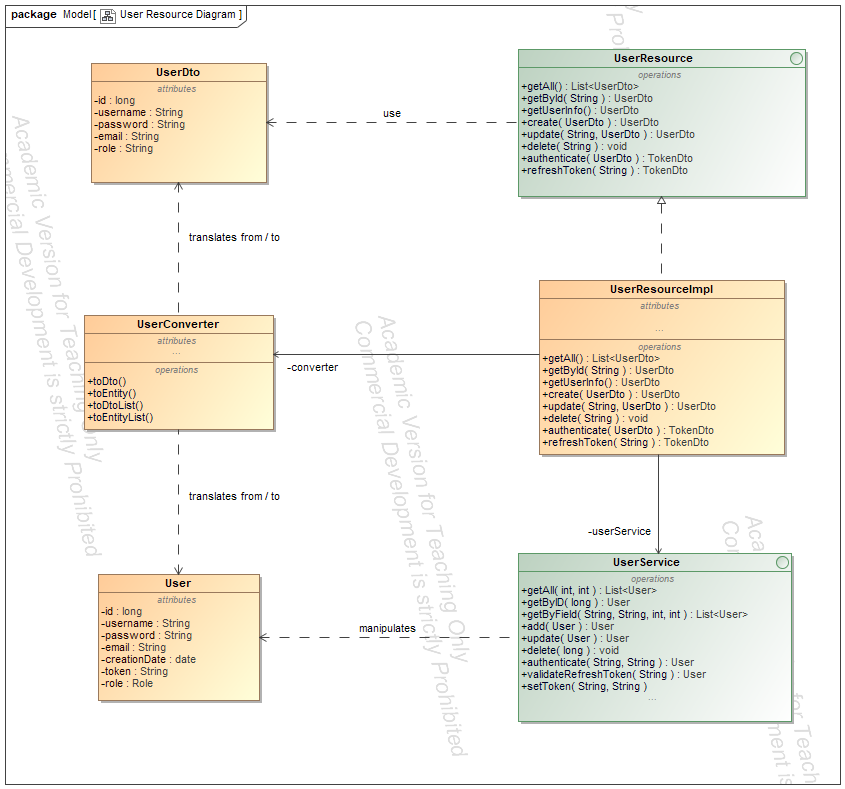
\includegraphics[
   keepaspectratio=true
]{./05_Diseno/disenorest.png}
\caption{Ejemplo servicios usuario}
\end{figure}


\begin{itemize}
	\item \textbf{UserDto: } Es el objeto de transferencia.
	\item \textbf{User: } Objeto de negocio para la entidad usuario.
	\item \textbf{UserResource: } Interfaz que expone ciertas funcionalidades a través de un recurso web. En este ejemplo, se define la implementación \textit{UserResourceImpl}, encargada de implementar las funciones establecidas en la interfaz. Los datos e información manejada se hace a través del objeto de transferencia.
	\item \textbf{UserService: } Servicio ofrecido por la capa modelo que gestiona los casos de uso y funcionalidades referentes a usuarios. Manipula el objeto de negocio \textit{User} y sus funcionalidades son invocadas por parte de \textit{UserResouceImpl}.
	\item \textbf{UserConverter: } Clase de utilidad que permite a la implementación del recurso \textit{UserResource} transformar el objeto de negocio en un objeto de transferencia, y viceversa.

\end{itemize}

El resto de servicios definidos en la aplicación seguirán una estructura similar. Se ofrecerán recursos web accesibles mediante HTTP que permitirán la invocación remota de la lógica de negocio de la aplicación.


\section{Capa Interfaz}
La capa interfaz, también conocida como capa cliente o capa de presentación, es la encargada de separar la interacción del usuario respecto a la lógica de negocio. Esta capa simplemente presenta la información al usuario y recibe las peticiones que debe comunicar a la capa modelo.

En nuestro sistema, existen dos presentaciones de la aplicación completamente diferentes e independientes: una aplicación web accesible desde navegador y una aplicación desarrollada para dispositivos móviles.

\subsection{Aplicación web}
La aplicación web se ejecutará en un servidor de aplicaciones que recibirá y gestionará todas las peticiones del cliente. Será la encargada de generar la vista web de la aplicación así como comunicarse con la capa modelo, accediendo a la capa de servicios del modelo.

Seguirá el patrón de arquitectura Modelo-Vista-Controlador (MVC).

\subsubsection*{Patrón Modelo-Vista-Controlador}
MVC es un patrón de arquitectura de software que separa los datos y la lógica de negocio, de su representación. Está formado por tres componentes distintos: modelo, vista y controlador.

El modelo es la información de la aplicación y el que proviene de la lógica de negocio. La vista, por su parte, es la representación en pantalla mientras que el controlador es el encargado de mantener la comunicación con el modelo y definir la forma en que la interfaz reacciona a las peticiones del usuario. Antes del patrón MVC, los diseños de interfaz de usuario tendían a agrupar estos objetos. Con este patrón se consigue desacoplar vistas y modelo estableciendo un protocolo de `suscripción-notificación' entre ellos.

\subsubsection*{Diagrama MVC aplicación web}
A continuación se mostrará un diagrama donde se verán los componentes MVC anteriormente comentados en el sistema de nuestra aplicación web.

\begin{figure}[H]
\centering
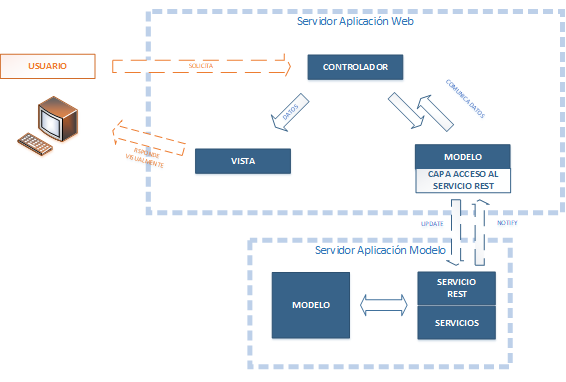
\includegraphics[
   keepaspectratio=true
]{./05_Diseno/mvccapaweb.png}
\caption{Diagrama MVC aplicación web}
\end{figure}

El controlador recibirá las solicitudes del usuario y obtendrá los datos del modelo a través del servicio REST especificado. Con estos datos, el controlador creará la vista correspondiente, que será entregada al usuario.


\subsubsection*{Diseño capa acceso al servicio}
En la siguiente figura se mostrará el diseño que permitirá invocar a la capa de servicios del modelo.
\begin{figure}[H]
\centering
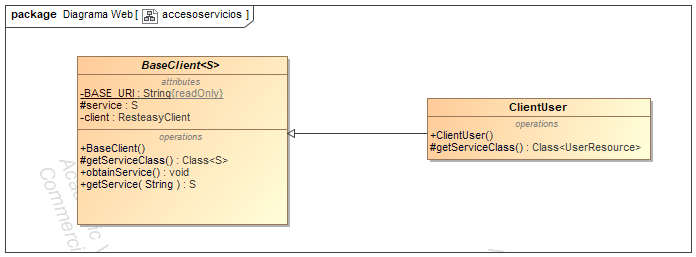
\includegraphics[
   keepaspectratio=true
]{./05_Diseno/accesoservicios.png}
\caption{Ejemplo acceso a servicios cliente web}
\end{figure}

En este diagrama se definen dos clases: \textit{BaseClient} y \textit{ClientRoute}. La primera es la encargada de crear un cliente que permita construir peticiones HTTP que se usarán para invocar los métodos ofrecidos en la capa de servicios.

Por su parte, la clase \textit{ClientRoute}, modifica el comportamiento de la clase anterior indicando sobre qué recurso tiene que elaborar las peticiones HTTP. En este ejemplo, se utiliza el recurso \textit{RouteResource} de la capa de servicios. Análogamente, se crean las diferentes clases clientes, para acceder a los diferentes recursos creados en la capa de servicios del modelo.

\subsubsection*{Diseño controladores}
\begin{figure}[H]
\centering
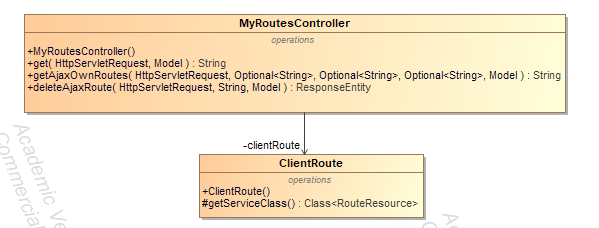
\includegraphics[
   keepaspectratio=true
]{./05_Diseno/controladorweb.png}
\caption{Ejemplo controlador cliente web}
\end{figure}

En este ejemplo se especifica el controlador \textit{MyRoutesController} que define sobre una URL los métodos que se pueden realizar para la gestión de las rutas propias de un usuario.
\begin{itemize}
	\item \textbf{ClientRoute: } Clase que permite invocar los métodos de la capa de servicios.
	\item \textbf{MyRoutesController: }Controlador web que ofrece las siguientes funcionalidades:
	\begin{itemize}
		\item \textbf{get: }Recibe las peticiones GET sobre la URL especificada.
		\item \textbf{getAjaxOwnRoutes: }Recibe las peticiones asíncronas para consultar las rutas propias.
		\item \textbf{deleteAjaxRoute: }Recibe las peticiones asíncronas para eliminar una ruta específica.
	\end{itemize}
\end{itemize}


\subsection{Aplicación móvil}
La aplicación móvil será desarrollada mediante el SDK Ionic. Una aplicación Ionic es, en esencia, una aplicación Angular que se base en una arquitectura Modelo-Vista-VistaModelo (MVVM).

\subsubsection*{Patrón Modelo-Vista-VistaModelo}
Este modelo se considera una adaptación del patrón anteriormente explicado, el Modelo-Vista-Controlador.

MVC y MVVM siguen un funcionamiento similar pero con unas pequeñas diferencias. 
\begin{itemize}
	\item En el patrón Modelo-Vista-Controlador se separan los datos de una aplicación en los tres componentes anteriormente mencionados (Modelo, Vista y Controlador). Cuando la lógica de negocio realiza un cambio, este es necesario que sea actualizado en la vista.
	
	\item El patrón Modelo-Vista-VistaModelo sigue la misma separación que el patrón MVC. En este caso, en vez de controlar los cambios manualmente en la vista o en los datos como sucede con el patrón MVC, estos se actualizan directamente cuando sucede un cambio o modificación en ellos. De tal manera, que si la vista actualiza un dato que está presentando, este se actualizaría en el modelo automáticamente, y viceversa.
\end{itemize}

El denominado `Controller' del patrón MVC cambia a 'ViewModel´ en el MVVM. Este último, a diferencia del anterior, incorpora un `binder' que se encarga de sincronizar la información entre la vista y el modelo.


\begin{figure}[H]
\centering
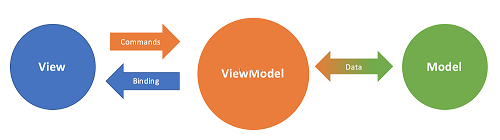
\includegraphics[
   keepaspectratio=true
]{./05_Diseno/mvvm.png}
\caption{Diagrama patrón MVVM}
\end{figure}


\subsubsection*{Diseño capa acceso al servicio}
\begin{figure}[H]
\centering
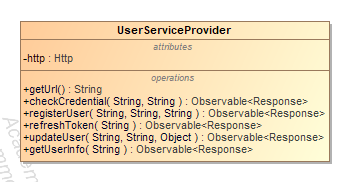
\includegraphics[
   keepaspectratio=true
]{./05_Diseno/accesoserviciosmov.png}
\caption{Ejemplo acceso servicios cliente móvil}
\end{figure}

Para el cliente móvil se definen un conjunto de clases que permitan ejecutar los métodos de la capa de servicios. \textit{UserServiceProvider} es una de ellas, en la que se crean y elaboran las peticiones HTTP necesarias para ejecutar los diferentes métodos ofrecidos por la capa servicios del modelo.


\subsubsection*{Diseño controladores}
\begin{figure}[H]
\centering
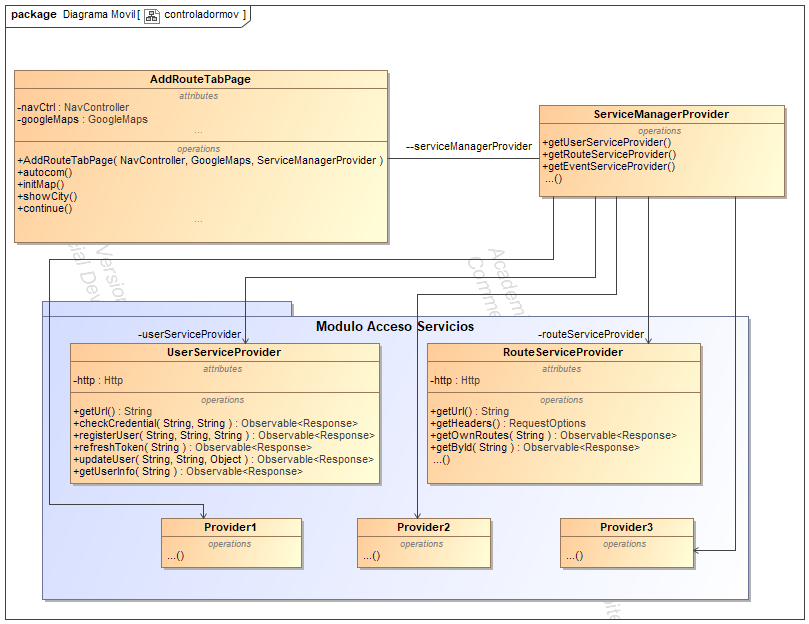
\includegraphics[
   keepaspectratio=true
]{./05_Diseno/controladormov.png}
\caption{Ejemplo controlador cliente móvil}
\end{figure}

En la figura 7.18 se muestra el ejemplo de un controlador de la aplicación móvil, \textit{AddRouteTabPage}, encargado de gestionar la pantalla que permite al usuario crear rutas. Dicho controlador hace uso de la clase \textit{ServiceManagerProvider} que permite obtener las diferentes clases que implementan la capa de acceso a los servicios.


\section{Diseño autenticación}
Uno de los principales aspectos de seguridad de las aplicaciones son los procesos de autenticación y de autorización. Para nuestras aplicaciones se propone el siguiente diseño basado en tokens de acceso (\textit{access tokens}) y tokens de refresco (\textit{refresh tokens}) para la autenticación y autorización de los usuarios. A continuación, se mostrará un diagrama de secuencia en el que se podrá observar el proceso de autenticación en el cliente móvil.


\begin{figure}[H]
\centering
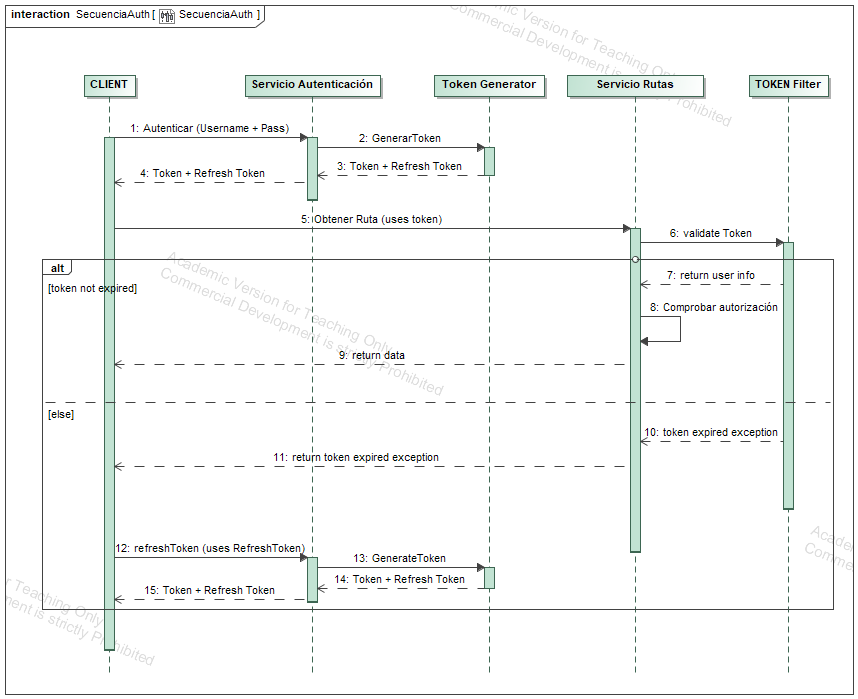
\includegraphics[
   keepaspectratio=true
]{./05_Diseno/SecuenciaAuth.png}
\caption{Ejemplo secuencia autenticación cliente móvil}
\end{figure}


Este diseño de autenticación surge debido al requisito funcional para el cliente móvil, que exige mantener la sesión abierta, sin necesidad de autenticarse de nuevo, cada vez que la aplicación es iniciada. Con este diseño, el cliente se autentica en la aplicación y consigue un token de acceso, con el que podrá realizar acciones autenticadas, y un token de refresco. Cuando el primero caduca y deja de ser válido en el tiempo, el sistema devuelve una excepción específica, de tal manera, que el cliente móvil, sabrá que tendrá que actualizar dicho token de acceso realizando una petición específica al servidor indicando su token de refresco. 

Con este procedimiento, se consigue que el cliente móvil, almacenando los tokens ofrecidos por el sistema, no tenga que solicitar al usuario las credenciales cada vez que el token de acceso deje de ser válido. Únicamente, solicitará las credenciales al usuario cuando no sea capaz de obtener uno nuevo mediante el servicio del token de refresco.

El cliente web seguirá el mismo proceso de autenticación mediante token de acceso pero, por las particularidades y características de dicho cliente, no hará uso del token de refresco. Cuando el token de acceso deje de ser válido, el sistema pedirá al usuario que introduzca de nuevo las credenciales.





